\documentclass[letterpaper]{article} % DO NOT CHANGE THIS
\usepackage{aaai2026}  % DO NOT CHANGE THIS
\usepackage{times}  % DO NOT CHANGE THIS
\usepackage{helvet}  % DO NOT CHANGE THIS
\usepackage{courier}  % DO NOT CHANGE THIS
\usepackage[hyphens]{url}  % DO NOT CHANGE THIS
\usepackage{graphicx} % DO NOT CHANGE THIS
\urlstyle{rm} % DO NOT CHANGE THIS
\def\UrlFont{\rm}  % DO NOT CHANGE THIS
\usepackage{natbib}  % DO NOT CHANGE THIS AND DO NOT ADD ANY OPTIONS TO IT
\usepackage{caption} % DO NOT CHANGE THIS AND DO NOT ADD ANY OPTIONS TO IT
\frenchspacing  % DO NOT CHANGE THIS
\setlength{\pdfpagewidth}{8.5in} % DO NOT CHANGE THIS
\setlength{\pdfpageheight}{11in} % DO NOT CHANGE THIS
\usepackage{amsmath}
\usepackage{amssymb}
\usepackage{booktabs}
\nocopyright

\pdfinfo{
/TemplateVersion (2026.1)
}

\setcounter{secnumdepth}{0}
\newcommand{\nmin}{n_{\min}}

\title{Pooled Covariance Shrinkage for HyCal: Few-Shot Cross-Domain\\Class-Incremental Learning}
\author{
Zhou Ziyue, He Xinyan, Zhang Yining, Xu Pengyang, Lu Wenrui, Hu Hangrui
}
\affiliations{
    AI6103 Deep Learning, Nanyang Technological University
}

\renewcommand{\topfraction}{0.9}
\renewcommand{\dbltopfraction}{0.9}
\renewcommand{\textfraction}{0.1}
\renewcommand{\floatpagefraction}{0.8}
\renewcommand{\dblfloatpagefraction}{0.8}
\setcounter{topnumber}{3}
\setcounter{dbltopnumber}{3}
\setcounter{totalnumber}{5}
\begin{document}
\maketitle

\begin{abstract}
Few-shot cross-domain class-incremental learning adds classes from different visual domains, each with only a few labelled support images. HyCal scores queries on frozen CLIP features by combining cosine similarity with a per-class Mahalanobis distance. With $K \in \{5, 10\}$ support images in a 512-dimensional fused space, each class covariance has rank at most $K$. We replace each class covariance with a mixture of itself (25\%) and the within-class covariance pooled over the current session (75\%), and leave prototypes, fusion, calibration and weighting unchanged. In paired comparisons that change only the shrinkage coefficient $\alpha$, mean test accuracy rises by 2.93 and 2.92 percentage points (pp) on EuroSAT RGB at 5 and 10 shots and by 1.71 and 4.00 pp on Galaxy10 DECaLS; 11 of the 12 paired runs improve. Applied without retuning to Flowers102 and OrganAMNIST, shrinkage improves all 12 paired runs (2.15 pp on Flowers102 at both shot counts; 4.92 and 6.02 pp on OrganAMNIST). We also find that the official balanced script ($\nmin = 20$) reduces HyCal to cosine-only scoring for $K \le 10$. In a two-domain test with 10 support images per EuroSAT class and one per Galaxy10 class, Mahalanobis-only scoring assigned 42.18\% of EuroSAT images to galaxy classes; weighted HyCal with shrinkage assigned 0.11\%.
\end{abstract}

\begin{figure*}[t]
\centering
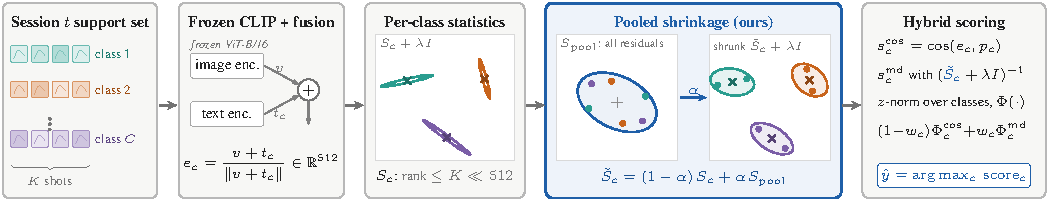
\includegraphics[width=\textwidth]{figures/fig_overview.pdf}
\caption{Overview. With $K \ll 512$ support images, each class covariance $S_c$ in HyCal's fused space is rank-deficient (needles; exact 2-D cartoon with two shots per class). We pool the within-class residuals of session $t$ into $S_{\mathrm{pool}}$ and shrink each $S_c$ toward it (blue); all other HyCal steps are unchanged.}
\label{fig:overview}
\end{figure*}

\begin{table*}[t]
\centering
\footnotesize
\setlength{\tabcolsep}{3pt}
\begin{tabular}{@{}llllccl@{}}
\toprule
Dataset & Role & Domain & Cls. & Size & Split (train / val / test) & Split source \\
\midrule
EuroSAT RGB \citep{helber2019eurosat} & Primary & Land cover & 10 & $64{\times}64$ & 13,500 / 5,400 / 8,100 & CoOp \citep{zhou2022coop} \\
Galaxy10 DECaLS \citep{galaxy10} & Primary & Galaxies & 10 & $256{\times}256$ & 14,188 / 1,774 / 1,774 & Stratified 80/10/10 \\
Flowers102 \citep{nilsback2008flowers} & Held-out & Flora & 102 & Var. & 4,093 / 1,633 / 2,463 & CoOp \citep{zhou2022coop} \\
OrganAMNIST \citep{yang2023medmnist} & Held-out & Abdominal CT & 11 & $224{\times}224$ & 34,561 / 6,491 / 17,778 & MedMNIST v2 official \\
\bottomrule
\end{tabular}
\caption{Datasets. EuroSAT and Galaxy10 were used to choose the configuration; Flowers102 and OrganAMNIST were used only for transfer. Grayscale OrganAMNIST slices are replicated to three channels for CLIP.}
\label{tab:data}
\end{table*}

\section{Introduction}

Few-shot class-incremental learning extends a classifier over a sequence of sessions, each adding new classes with a few labelled support images. At inference, all classes seen so far share one label space. In the cross-domain setting, sessions bring classes from different visual domains, such as satellite images, galaxy surveys, flower photographs and CT scans, and the classifier receives no domain label.

HyCal \citep{lee2026hycal} keeps CLIP \citep{radford2021clip} frozen and stores a prototype and a sample covariance for each class in an image--text fused space. At test time it calibrates cosine similarity and Mahalanobis distance across the candidate classes and combines them with a weight that depends on the number of support images. Each session adds statistics for its new classes and leaves earlier statistics unchanged. We used the official implementation \citep{hycalcode} at commit 4558fb7.

With $K \in \{5, 10\}$, each class covariance $S_c \in \mathbb{R}^{512 \times 512}$ has rank at most $K$, so in about 500 directions the variance comes only from the ridge term $\lambda I$. Following classical covariance shrinkage \citep{friedman1989,ledoit2004}, we pool within-class residuals over all classes of the current session and shrink each class covariance toward this pooled estimate (Figure~\ref{fig:overview}). The change adds one scalar parameter, $\alpha$, and needs no stored images from earlier sessions.

Our contributions are:
\begin{enumerate}
\item Session-level pooled covariance shrinkage for HyCal, which improved 23 of 24 paired five- and ten-shot runs across four domains, including two domains not used to choose the configuration.
\item The observation that the official balanced script (\texttt{run\_balanced.sh}, $\nmin = 20$) switches off Mahalanobis scoring for $K \le 10$, and a control that differs from our method only in $\alpha$.
\item Per-class results on the transfer domains and a two-domain analysis of cross-domain errors when the domains have different shot counts.
\end{enumerate}


\begin{table}[t]
\centering
\small
\setlength{\tabcolsep}{4pt}
\begin{tabular}{@{}lcccc@{}}
\toprule
Configuration & $\lambda$ & $\nmin$ & scale & $\alpha$ \\
\midrule
Zero-shot (CLIP prompts) & -- & -- & -- & -- \\
Official (\texttt{run\_balanced.sh}) & $10^{-4}$ & 20 & 5 & 0 \\
Baseline (CLI default) & $10^{-4}$ & 5 & 5 & 0 \\
Tuned HyCal (control) & $10^{-4}$ & 2 & 1 & 0 \\
Shrinkage (ours) & $10^{-4}$ & 2 & 1 & 0.75 \\
\bottomrule
\end{tabular}
\caption{Scoring configurations compared. Shrinkage and Tuned HyCal differ solely in $\alpha$.}
\label{tab:configs}
\end{table}

\begin{table*}[t]
\centering
\footnotesize
\setlength{\tabcolsep}{4pt}
\begin{tabular}{@{}lrrrrrrrrr@{}}
\toprule
Dataset & $K$ & \shortstack{Zero-\\shot} & \shortstack{Cosine\\(= Official)} & \shortstack{MD-\\only} & \shortstack{Baseline\\($\nmin{=}5$)} & \shortstack{Tuned HyCal\\($\alpha{=}0$)} & \shortstack{Shrinkage\\($\alpha{=}0.75$)} & \shortstack{Paired gain\\(pp)} & Wins \\
\midrule
EuroSAT & 5 & 38.67 & 71.37 $\pm$ 1.97 & 76.67 $\pm$ 1.32 & 74.09 $\pm$ 2.13 & 76.60 $\pm$ 1.63 & \textbf{79.53 $\pm$ 1.30} & \textbf{+2.93 $\pm$ 1.24} & 3/3 \\
EuroSAT & 10 & 38.67 & 75.67 $\pm$ 0.92 & 83.47 $\pm$ 1.01 & 82.07 $\pm$ 0.99 & 83.49 $\pm$ 1.01 & \textbf{86.40 $\pm$ 0.87} & \textbf{+2.92 $\pm$ 0.25} & 3/3 \\
Galaxy10 & 5 & 9.81 & 37.99 $\pm$ 1.81 & 37.82 $\pm$ 2.25 & 38.61 $\pm$ 1.44 & 37.99 $\pm$ 2.03 & \textbf{39.70 $\pm$ 2.04} & \textbf{+1.71 $\pm$ 2.76} & 2/3 \\
Galaxy10 & 10 & 9.81 & 40.00 $\pm$ 1.95 & 39.74 $\pm$ 0.65 & 41.06 $\pm$ 0.61 & 39.74 $\pm$ 0.70 & \textbf{43.74 $\pm$ 1.77} & \textbf{+4.00 $\pm$ 1.08} & 3/3 \\
\bottomrule
\end{tabular}
\caption{Primary test accuracy (\%, mean $\pm$ std over 3 seeds). Official (\texttt{run\_balanced.sh}, $\nmin=20$) equals Cosine-only for $K \le 10$. Paired gain = Shrinkage $-$ Tuned HyCal on the same seed. At $K = 1$, all few-shot variants reduce to cosine scoring: $52.78 \pm 5.96\%$ (EuroSAT) and $24.31 \pm 8.24\%$ (Galaxy10).}
\label{tab:main}
\end{table*}

\section{Background and Method}

\subsection{HyCal Preliminaries}

A frozen CLIP ViT-B/16 encoder \citep{radford2021clip} maps an image to a unit vector $v \in \mathbb{R}^{512}$ and each candidate class prompt to a unit vector $t_c \in \mathbb{R}^{512}$. HyCal \citep{lee2026hycal} fuses them for each candidate class:
\begin{equation}
e_c = \frac{v + t_c}{\lVert v + t_c \rVert}.
\label{eq:fusion}
\end{equation}
For class $c$ with $K_c$ support images, HyCal computes the fused support vectors $\{e_{c,i}\}_{i=1}^{K_c}$, the normalised prototype $p_c = \bar{e}_c / \lVert \bar{e}_c \rVert$ with $\bar{e}_c = \frac{1}{K_c}\sum_{i=1}^{K_c} e_{c,i}$, and the sample covariance around $p_c$:
\begin{equation}
S_c = \frac{1}{K_c - 1} \sum_{i=1}^{K_c} (e_{c,i} - p_c)(e_{c,i} - p_c)^\top \quad (K_c > 1),
\label{eq:cov}
\end{equation}
with $S_c = 10^{-3} I$ when $K_c = 1$ \citep{hycalcode}.

Each candidate class receives a cosine score and a regularised Mahalanobis score, with default ridge $\lambda = 10^{-4}$:
\begin{equation}
\begin{split}
s^{\mathrm{cos}}_c &= \cos(e_c, p_c),\\
s^{\mathrm{md}}_c &= -(e_c - p_c)^\top (S_c + \lambda I)^{-1} (e_c - p_c).
\end{split}
\label{eq:scores}
\end{equation}
The official relative Mahalanobis distance also subtracts a background term that is the same for every candidate class of a query, so it cancels in the per-query $z$-normalisation. Each score is $z$-normalised across the candidate classes, mapped through the Gaussian CDF $\Phi$, and combined:
\begin{equation}
\begin{split}
\mathrm{score}_c &= (1 - w_c)\,\Phi(z^{\mathrm{cos}}_c) + w_c\,\Phi(z^{\mathrm{md}}_c),\\
w_c &= \mathbb{I}[K_c \ge \nmin]\,\mathrm{sigmoid}\!\left(\frac{K_c - \nmin}{\mathrm{scale}}\right).
\end{split}
\label{eq:combine}
\end{equation}
Classes with $K_c < \nmin$ get $w_c = 0$ and are scored by cosine similarity alone.

\begin{table}[t]
\centering
\footnotesize
\setlength{\tabcolsep}{2.5pt}
\begin{tabular}{@{}lrccc@{}}
\toprule
Dataset & $K$ & $\alpha{=}0$ & $\alpha{=}0.75$ & Gain (pp) \\
\midrule
Flowers102 & 5 & 93.26 $\pm$ 0.19 & \textbf{95.41 $\pm$ 0.44} & +2.15 $\pm$ 0.31 \\
Flowers102 & 10 & 95.02 $\pm$ 0.35 & \textbf{97.17 $\pm$ 0.34} & +2.15 $\pm$ 0.36 \\
OrganAMNIST & 5 & 59.37 $\pm$ 0.53 & \textbf{64.30 $\pm$ 0.77} & +4.92 $\pm$ 0.59 \\
OrganAMNIST & 10 & 65.61 $\pm$ 1.44 & \textbf{71.63 $\pm$ 1.88} & +6.02 $\pm$ 1.18 \\
\bottomrule
\end{tabular}
\caption{Zero-retuning transfer to held-out domains (\%, mean $\pm$ std over 3 seeds; 3/3 seeds improved in every row). At $K=1$, both settings are identical: $70.35 \pm 1.07\%$ (Flowers102) and $45.47 \pm 3.81\%$ (OrganAMNIST).}
\label{tab:transfer}
\end{table}

\begin{table*}[t]
\centering
\small
\begin{tabular}{@{}lrcccc@{}}
\toprule
Dataset & $K$ & Lower threshold & Raise $\lambda$ & Add shrinkage & Add shrinkage \\
 & & {\footnotesize $\nmin\ 5{\to}2$, scale $5{\to}1$} & {\footnotesize $10^{-4}{\to}10^{-3}$} & {\footnotesize $\lambda = 10^{-4}$} & {\footnotesize $\lambda = 10^{-3}$} \\
\midrule
EuroSAT & 5 & +2.51 $\pm$ 0.53 (3/3) & $-$0.04 $\pm$ 0.16 (1/3) & \textbf{+2.93 $\pm$ 1.24} (3/3) & +2.56 $\pm$ 0.87 (3/3) \\
EuroSAT & 10 & +1.42 $\pm$ 0.44 (3/3) & $-$0.04 $\pm$ 0.51 (2/3) & \textbf{+2.92 $\pm$ 0.25} (3/3) & +1.68 $\pm$ 0.48 (3/3) \\
Galaxy10 & 5 & $-$0.62 $\pm$ 0.99 (1/3) & +0.39 $\pm$ 0.77 (2/3) & \textbf{+1.71 $\pm$ 2.76} (2/3) & +1.39 $\pm$ 0.68 (3/3) \\
Galaxy10 & 10 & $-$1.32 $\pm$ 0.60 (0/3) & +1.18 $\pm$ 0.26 (3/3) & \textbf{+4.00 $\pm$ 1.08} (3/3) & +1.95 $\pm$ 0.27 (3/3) \\
\bottomrule
\end{tabular}
\caption{Ablation of scoring threshold/scale, ridge strength $\lambda$, and covariance shrinkage ($\alpha = 0.75$). Paired gains in pp, mean $\pm$ std over 3 seeds (seeds improved).}
\label{tab:ablation}
\end{table*}

\subsection{Pooled Covariance Shrinkage}

We pool the residuals of all multi-shot classes $\mathcal{C}_t^{+} = \{c \in \mathcal{C}_t : K_c > 1\}$ in the current session $t$, each centred on its own prototype:
\begin{equation}
S_{\mathrm{pool}} = \frac{\sum_{c \in \mathcal{C}_t^{+}} \sum_{i=1}^{K_c} (e_{c,i} - p_c)(e_{c,i} - p_c)^\top}{\sum_{c \in \mathcal{C}_t^{+}} (K_c - 1)}.
\label{eq:spool}
\end{equation}
Centring on each class's own prototype keeps differences between class means out of $S_{\mathrm{pool}}$. The degrees of freedom rise from $K_c - 1$ to $\sum_{c \in \mathcal{C}_t^{+}} (K_c - 1)$, which is $C(K-1)$ in a balanced session of $C$ classes. Pooling uses only the classes of session $t$, so earlier sessions need no stored images and no updates.

Each class covariance is shrunk toward $S_{\mathrm{pool}}$,
\begin{equation}
\tilde{S}_c = (1 - \alpha)\, S_c + \alpha\, S_{\mathrm{pool}}, \quad \alpha \in [0, 1],
\label{eq:shrink}
\end{equation}
and $\tilde{S}_c$ replaces $S_c$ in the Mahalanobis score of Eq.~\eqref{eq:scores}, which becomes $-(e_c - p_c)^\top (\tilde{S}_c + \lambda I)^{-1} (e_c - p_c)$. Prototypes, cosine scores, fusion, $z$-normalisation and weighting are the same as in HyCal. One-shot classes skip shrinkage and, with $\nmin = 2$, get $w_c = 0$, so one-shot predictions equal cosine scoring. If a session has only one multi-shot class ($|\mathcal{C}_t^{+}| = 1$), then $S_{\mathrm{pool}} = S_c$ and the method reduces to HyCal for every $\alpha$.

We chose $(\alpha, \lambda, \nmin, \mathrm{scale})$ jointly on the validation splits of EuroSAT and Galaxy10, using mean accuracy over $K \in \{1, 5, 10\}$ and three support seeds. The selected values are $\alpha = 0.75$, $\lambda = 10^{-4}$, $\nmin = 2$ and $\mathrm{scale} = 1$, under which $w_c$ is close to 1 at 5 and 10 shots. Mean validation accuracy was 53.07\% at $\alpha = 0$ and 54.56\%, 54.62\%, 54.63\% and 54.49\% at $\alpha = 0.25, 0.5, 0.75$ and $1$. All four values were fixed before the test evaluation and the transfer runs. Setting $\alpha = 0$ with the same $\lambda$, $\nmin$ and scale gives the control, Tuned HyCal.

\begin{figure}[t]
\centering
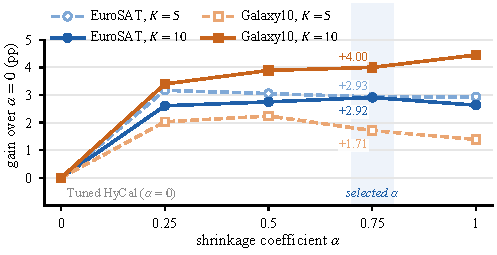
\includegraphics[width=\columnwidth]{figures/fig_alpha.pdf}
\caption{Test accuracy gain over $\alpha = 0$ (3-seed means; $\lambda = 10^{-4}$, $\nmin = 2$, scale $= 1$). Labels: paired gains at the validation-selected $\alpha = 0.75$.}
\label{fig:alpha}
\end{figure}

\begin{table}[t]
\centering
\small
\setlength{\tabcolsep}{3.5pt}
\begin{tabular}{@{}lcc@{}}
\toprule
Scoring modification & 5-shot (\%) & 10-shot (\%) \\
\midrule
Query-gated weighting & 73.87 $\pm$ 2.29 & 82.62 $\pm$ 1.16 \\
\quad (vs.\ uniform weight $\times 1.5$) & {\footnotesize (+0.27 $\pm$ 0.03)} & {\footnotesize (+0.69 $\pm$ 0.20)} \\
Projected shared visual cov. & \textbf{79.68 $\pm$ 0.98} & 86.18 $\pm$ 0.73 \\
Pooled cov.\ shrinkage (ours) & 79.53 $\pm$ 1.30 & \textbf{86.40 $\pm$ 0.87} \\
\bottomrule
\end{tabular}
\caption{Alternatives on the same EuroSAT support sets and test images. Query gating keeps its OrganAMNIST settings ($\lambda = 10^{-3}$, MD from 3 shots); brackets: paired gain (pp).}
\label{tab:alternatives}
\end{table}

\begin{figure}[t]
\centering
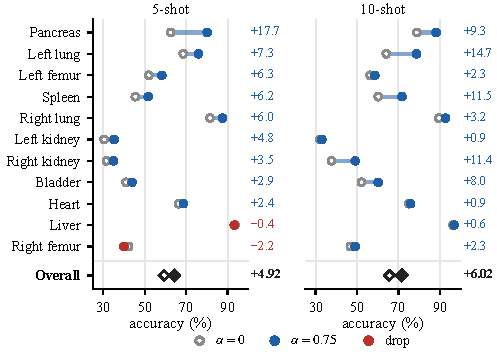
\includegraphics[width=\columnwidth]{figures/fig_organ.pdf}
\caption{OrganAMNIST per-class test accuracy (3-seed mean), $\alpha = 0$ (open) vs.\ $\alpha = 0.75$ (filled), sorted by 5-shot gain; right: gains in pp.}
\label{fig:organ}
\end{figure}

\section{Experimental Setup}

Table~\ref{tab:data} lists the four datasets. All runs use the same frozen CLIP ViT-B/16 encoder, the official evaluation preprocessing (bicubic resize to 224 pixels, 224-pixel centre crop, CLIP normalisation, no augmentation), the official prompt templates, and cached float32 L2-normalised features. On EuroSAT at 5 shots with seed 0, our cached-feature implementation and the official \texttt{experiment\_runner.py} \citep{hycalcode} gave identical predictions on all 8,100 test images under cosine, Mahalanobis and weighted scoring.

Support sets are drawn from each training split for $K \in \{1, 5, 10\}$ with seeds 0, 1 and 42, and every method uses the same sets. We report top-1 test accuracy as the mean $\pm$ sample standard deviation over the three seeds, and paired gains in percentage points (pp) computed seed by seed. Table~\ref{tab:configs} lists the scoring configurations; we also report cosine-only and Mahalanobis-only scoring. With cached features, fitting a session and scoring the full test set takes under 0.5 s per run on a CPU.

\begin{table}[t]
\centering
\footnotesize
\setlength{\tabcolsep}{3pt}
\begin{tabular}{@{}lcc@{}}
\toprule
Scoring ($K_E{=}10, K_G{=}1$) & EuroSAT (\%) & E$\to$G (\%) \\
\midrule
Cosine-only / Official ($\nmin{=}20$) & 75.67 $\pm$ 0.92 & 0.00 \\
Mahalanobis-only & 51.93 $\pm$ 2.21 & 42.18 $\pm$ 3.11 \\
Baseline weighted ($\nmin{=}5$) & 83.37 $\pm$ 0.95 & 0.01 \\
Best unshrunk ($\lambda{=}10^{-3}$) & 83.44 $\pm$ 1.16 & 0.00 \\
Shrinkage ($\lambda{=}10^{-4}$) & \textbf{86.36 $\pm$ 0.85} & 0.11 \\
\bottomrule
\end{tabular}
\caption{Final-session two-domain incremental results (20 candidate classes) with unequal shots ($K_E = 10, K_G = 1$). The last two rows use $\nmin = 2$ and scale $= 1$, with $\alpha = 0$ and $\alpha = 0.75$. Galaxy10 accuracy is $24.31 \pm 8.24\%$ with $0.00\%$ G$\to$E error for all cosine/weighted rules.}
\label{tab:cross}
\end{table}

\section{Results}

\subsection{EuroSAT and Galaxy10}

Because \texttt{run\_balanced.sh} sets $\nmin = 20$, $w_c$ in Eq.~\eqref{eq:combine} is zero for every $K \le 10$, and the Official configuration gives the same predictions as cosine-only scoring (Table~\ref{tab:main}). The command-line default ($\nmin = 5$, Baseline) turns Mahalanobis scoring on and raises accuracy by 2.72 and 6.40 pp on EuroSAT and by 0.62 and 1.06 pp on Galaxy10 at 5 and 10 shots. Zero-shot CLIP reaches 38.67\% on EuroSAT and 9.81\% on Galaxy10, where it assigns 92\% of queries to one class.

Against Tuned HyCal ($\alpha = 0$), shrinkage ($\alpha = 0.75$) raises mean test accuracy in all four 5- and 10-shot settings and improves 11 of the 12 paired runs. On EuroSAT it adds $2.93 \pm 1.24$ pp at 5 shots and $2.92 \pm 0.25$ pp at 10 shots, improving every seed. On Galaxy10, Mahalanobis-only scoring without shrinkage is slightly below cosine-only (37.82\% against 37.99\% at 5 shots; 39.74\% against 40.00\% at 10 shots), and Tuned HyCal does not exceed cosine-only (37.99\% and 39.74\%). Shrinkage raises Galaxy10 accuracy by $4.00 \pm 1.08$ pp at 10 shots, on all three seeds. At 5 shots the mean gain is $1.71 \pm 2.76$ pp, and one of the three seeds decreases.

\subsection{Transfer to Flowers102 and OrganAMNIST}

We applied the fixed configuration without retuning to Flowers102 (102 flower classes) and OrganAMNIST (11 abdominal CT classes). Shrinkage improves all 12 paired runs (Table~\ref{tab:transfer}). On Flowers102, accuracy rises by 2.15 pp at both 5 shots (93.26\% to 95.41\%) and 10 shots (95.02\% to 97.17\%), with standard deviations of the gain at or below 0.36 pp. On OrganAMNIST, it rises by $4.92 \pm 0.59$ pp at 5 shots (59.37\% to 64.30\%) and $6.02 \pm 1.18$ pp at 10 shots (65.61\% to 71.63\%).

\subsection{Ablation}

Table~\ref{tab:ablation} separates the weighting settings, the ridge strength and shrinkage. Changing $\nmin$ from 5 to 2 and scale from 5 to 1 together raised mean accuracy on EuroSAT (2.51 and 1.42 pp) and lowered it on Galaxy10 (0.62 and 1.32 pp). Raising $\lambda$ from $10^{-4}$ to $10^{-3}$ raised Galaxy10 accuracy by 0.39 and 1.18 pp and changed EuroSAT by $-0.04$ pp. Shrinkage raised mean accuracy on both datasets at both ridge values, with larger gains at $\lambda = 10^{-4}$. At $\lambda = 10^{-4}$, every $\alpha \in \{0.25, 0.5, 0.75, 1\}$ beat $\alpha = 0$ in all four settings by 1.39 to 4.45 pp (Figure~\ref{fig:alpha}), while the spread across these four values was at most 0.30 pp on EuroSAT and 1.05 pp on Galaxy10.

\subsection{Alternative Scoring Designs}

Before settling on pooled shrinkage, we tried two other scoring changes (Table~\ref{tab:alternatives}). Projected shared visual covariance estimates one covariance in CLIP's visual space, similar to GDA \citep{wang2024gda}, and propagates it through the fusion step; on Flowers102, DTD \citep{cimpoi2014dtd} and FGVC-Aircraft \citep{maji2013aircraft} it gained 0.29, 0.04 and 0.09 pp over GDA at 5 shots. Query-gated weighting raises the Mahalanobis weight for queries whose top two cosine scores are close; on EuroSAT it gained $0.27 \pm 0.03$ and $0.69 \pm 0.20$ pp over raising the weight uniformly, on every seed. On EuroSAT, projected shared covariance led pooled shrinkage by 0.15 pp at 5 shots and trailed it by 0.22 pp at 10 shots, both within the 0.7 to 1.3 pp seed standard deviations, while query gating stayed 3.8 to 5.7 pp lower. We kept pooled shrinkage because it matches projected shared covariance while leaving HyCal's feature fusion unchanged, so the control differs from our method only in $\alpha$.

\section{Analysis}

\subsection{Per-Class Effects of Shrinkage}

Figure~\ref{fig:organ} gives OrganAMNIST accuracy per organ, averaged over three seeds. Shrinkage improved 9 of 11 organs at 5 shots, with the largest gains on pancreas (17.7 pp), left lung (7.3 pp) and left femur (6.3 pp), and all 11 organs at 10 shots, led by left lung (14.7 pp), spleen (11.5 pp) and right kidney (11.4 pp). Liver and right femur dropped by 0.4 and 2.2 pp at 5 shots. On Flowers102, shrinkage improved 62 classes, left 34 unchanged and lowered 6 at 5 shots; at 10 shots the counts were 60, 36 and 6.

On Galaxy10 at 5 shots, the gain varied most across seeds. There, $S_{\mathrm{pool}}$ rests on $C(K-1) = 40$ degrees of freedom, against 90 at 10 shots and 408 on Flowers102 at 5 shots. EuroSAT at 5 shots has the same 40 degrees of freedom and improved on every seed, so the pooled sample size alone does not account for the Galaxy10 result. Galaxy10 also has the lowest accuracy of the four domains, and its Disturbed and Merging classes stay at 20--27\%.

\subsection{Cross-Domain Incremental Evaluation}

We ran EuroSAT and Galaxy10 as a two-session incremental task, with 20 candidate classes in the final session, under both arrival orders and six shot combinations ($K_E / K_G \in \{5/5, 10/10, 10/1, 1/10, 10/5, 5/10\}$).

At 5/5 and 10/10 shots, no test image was assigned to the other domain's classes under any method. Shrinkage reached 79.41\% and 86.42\% on EuroSAT and 39.93\% and 43.76\% on Galaxy10, within 0.25 pp of the single-domain results; the $z$-normalisation now runs over 20 classes instead of 10. Swapping the arrival order left every final accuracy unchanged to two decimal places. The old-domain drop $F(d) = \max_u A(u, d) - A(T, d)$ was zero for cosine and Mahalanobis scoring and at most 0.21 pp for weighted HyCal.

With 10 shots for EuroSAT and 1 for Galaxy10 (Table~\ref{tab:cross}), Mahalanobis-only scoring assigned 42.18\% of EuroSAT test images to Galaxy10 classes, and EuroSAT accuracy fell to 51.93\%, 31.5 pp below its single-domain Mahalanobis-only result of 83.47\%. The two kinds of covariance differ in scale. A 10-shot class has rank at most 10, so about 500 directions carry variance $\lambda = 10^{-4}$, whereas the one-shot fallback gives $S_c + \lambda I = 1.1 \times 10^{-3} I$, 11 times larger in every direction. For EuroSAT queries, the median squared Mahalanobis distance was 274 to the true class and 287 to the nearest galaxy class, while the cosine similarities were 0.978 and 0.842.

Weighted HyCal gives one-shot classes $w_c = 0$, so they are scored by cosine similarity. With shrinkage, cross-domain errors stayed at or below 0.11\% across all six shot combinations, and EuroSAT accuracy in the 10/1 setting was 86.36\%, 2.92 pp above the best unshrunk configuration ($\lambda = 10^{-3}$, 83.44\%).

\section{Limitations}

\begin{itemize}
\item We chose the configuration on the EuroSAT and Galaxy10 validation splits and applied it unchanged to Flowers102 and OrganAMNIST. The ablations in Table~\ref{tab:ablation} and the error analyses were run on the test splits after this choice.
\item For each setting, we used three support seeds and counted how many paired runs showed higher accuracy with shrinkage. Three paired runs are too few for a formal significance test, and the Galaxy10 5-shot gain ($1.71 \pm 2.76$ pp) is still within seed-to-seed variation.
\item Our incremental evaluation covers two RGB domains and 20 classes; the HyCal paper reports eight domains \citep{lee2026hycal}.
\end{itemize}

\section{Conclusion}

Shrinking each HyCal class covariance toward the within-class covariance pooled over the current session adds one scalar, needs no retraining or stored images, and improved 23 of 24 paired 5- and 10-shot runs across four domains, two of them used without retuning. It also keeps cross-domain errors at or below 0.11\% when domains arrive with unequal shot counts. Future work includes setting $\alpha$ per session from the pooled degrees of freedom \citep{ledoit2004}, pooling across sessions from stored statistics alone, and evaluating on HyCal's full eight-domain benchmark with more seeds.

\bibliography{refs}

\end{document}
